\begin{figure}[t]
    \centering
    \begin{subfigure}[b]{0.45\textwidth}
    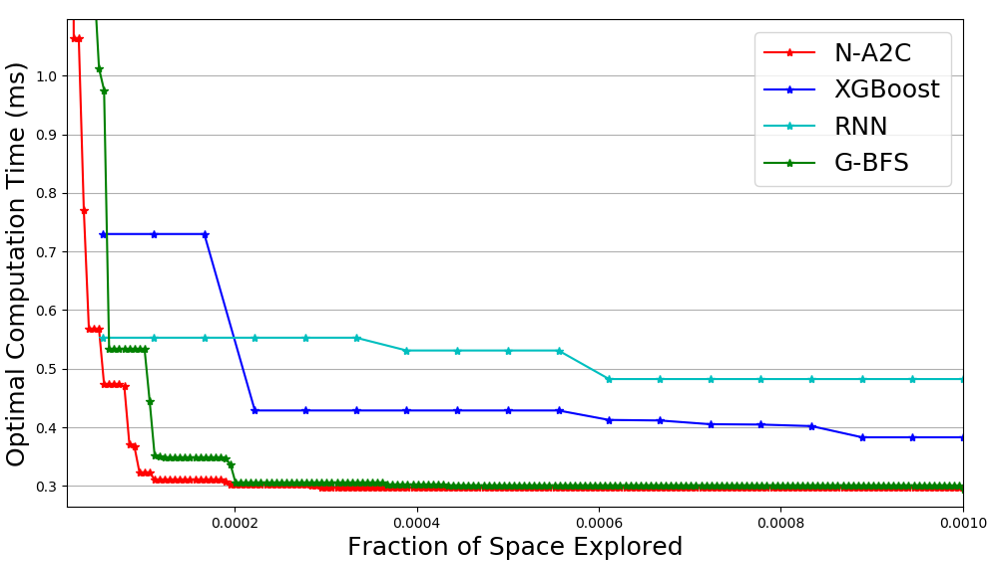
\includegraphics[width=\linewidth]{5_Simu/simu_11.png}
    \caption{Optimal computation time versus ratio of visited data}
    \label{fig:simu11}
    \end{subfigure}
    \hspace{0.2in}
    \begin{subfigure}[b]{0.45\textwidth}
    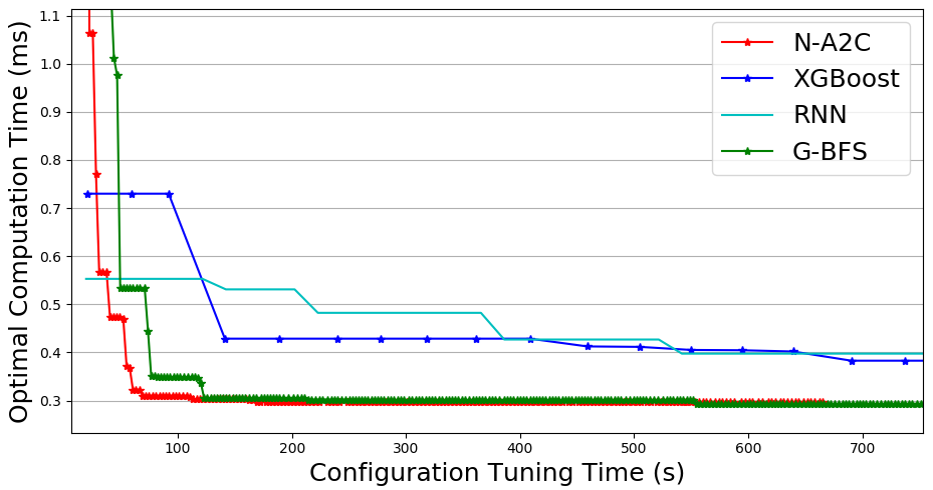
\includegraphics[width=\linewidth]{5_Simu/simu_12.png}
    \caption{Optimal computation time versus searching time}
    \label{fig:simu12}
    \end{subfigure}
    \caption{GEMM configuration tuning in (1024, 1024, 1024)}
    \label{fig:1024}
\end{figure}




Performance of the proposed GEMM configuration tuning approaches is evaluated in the TVM framework on Nvidia Titan Xp GPU. Following similar settings in TVM for GPUs, we set the number of nested loops for each dimension as $d_m=4, d_k=2, d_n=4$. We set the random selection parameter $\rho=5$ for the G-BFS method, and the maximum search step $\mathcal{T} =3$ for the N-A2C method. For generality, we set the initial state for the proposed methods as $s_0 = [[m,1,1,1],[k,1],[n,1,1,1]]$, referring to the situation without multi-level matrix tiling, and the performance of our proposed methods can be further improved by setting the initial state to a more meaningful configuration. In order to investigate the performance of our proposed methods, we compare them with the state-of-the-art algorithms including the XGBoost guided configuration tuning methods (or "the XGBoost method") in TVM framework and the general configuration optimization method using a RNN controller by Google researchers. Without specific explanations, the computation time for each configuration is the arithmetic mean for 10 repeated trials on the tested GPU hardware.

In simulations, we evaluate and compare the configuration tuning efficiency in a perceptron network, which is the fundamental unit for state-of-the-art neural network architectures and mainly includes GEMM for computation. During training of the network, we denote the setting of neural network in the format of $(number_of_inputs,batch_size,number_of_outputs)$, which corresponds to $(m,k,n)$ in matrices $A(m \times k)$ and $B(k \times n)$ for GEMM.

% In Fig. \ref{fig:1024}, we set the size of matrices $A(m \times k)$ and $B(k \times n)$ as $m=1024, k=1024, n=1024$

In Fig. \ref{fig:1024}, we set $number_of_inputs=1024$, $batch_size=1024$ and $number_of_outputs=1024$, and show the performance of our proposed configuration tuners. We first analyze the optimal computation time discovered with respect to the fraction of visited configurations in Fig. \ref{fig:simu11}. Based on the sizes of matrices and the number of nested loops, there are totally $899756$ configuration candidates. With the value of visited fraction increasing, the optimal computation time discovered generally decreases. Compared with the XGBoost and RNN methods, the proposed N-A2C and G-BFS methods are able to discover the configuration candidate with lower fraction of visited configuration candidates. Fig. \ref{fig:simu12} plots the optimal cost (hardware computation time) discovered by the four methods as tuning progresses over time. The proposed N-A2C and G-BFS methods generally use less tuning time to find the configuration with lower cost, compared with the XGBoost and RNN methods.

\begin{figure}[t]
    \centering
    \begin{subfigure}[b]{0.42\textwidth}
    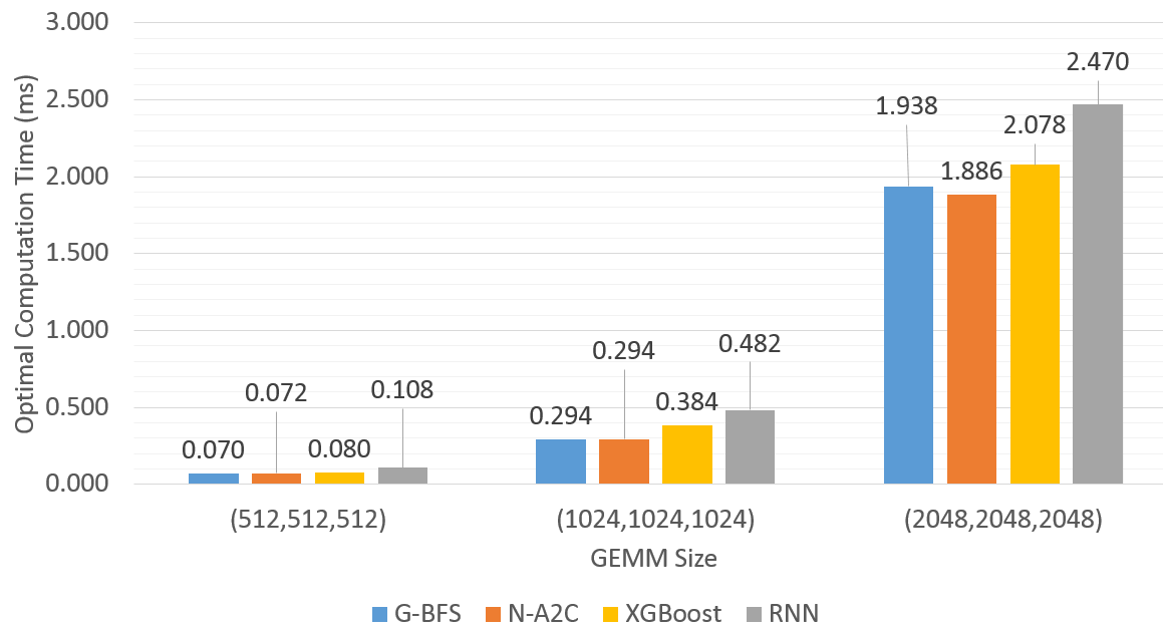
\includegraphics[width=\linewidth]{5_Simu/simu_21.png}
    \caption{When the fraction of visited configurations reaches 0.1\%}
    \label{fig:simu21}
    \end{subfigure}
    \hspace{0.2in}
    \begin{subfigure}[b]{0.42\textwidth}
    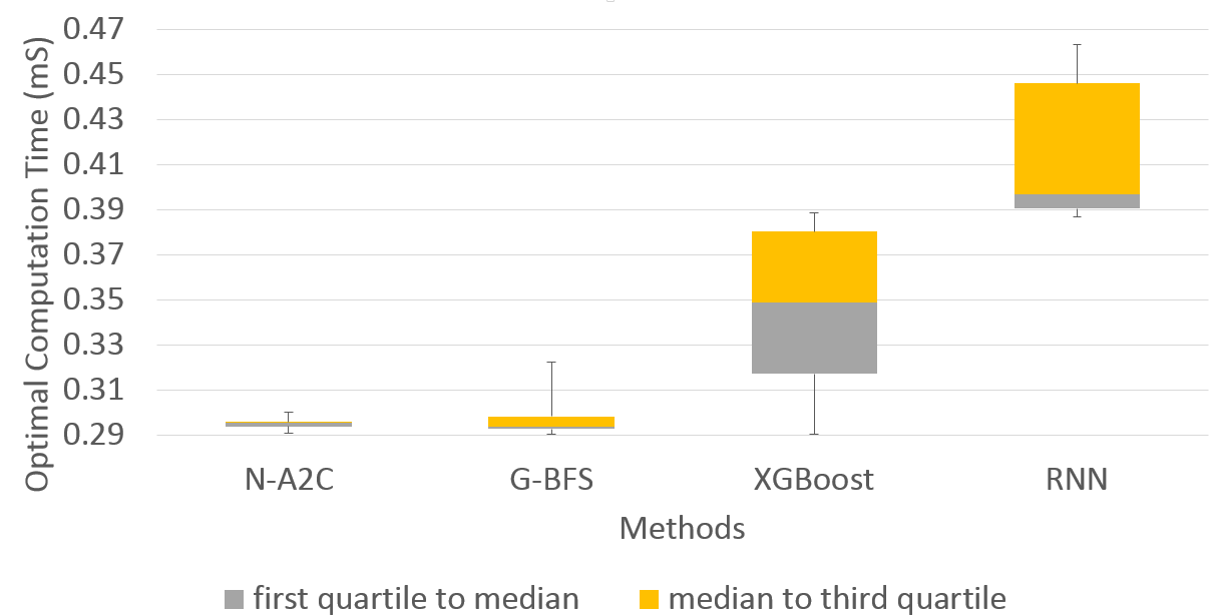
\includegraphics[width=\linewidth]{5_Simu/simu_23.png}
    \caption{When the tuning time reaches 750 seconds}
    \label{fig:simu23}
    \end{subfigure}
    \caption{Comparisons of configuration tuning efficiency}
    \label{fig:multi_case}
\end{figure}


In Fig. \ref{fig:multi_case}, we evaluate and compare the configuration tuning efficiency in the perceptron network. In Fig. \ref{fig:simu21}, we compare the discovered optimal computation time when the fraction of visited configuration candidates reaches 0.1\%. The total numbers of configuration candidates for $(512, 512, 512)$, $(1024, 1024, 1024)$, $(2048, 2048, 2048)$ matrix tiling are $484000$, $899756$ and $1589952$, respectively. As the sizes of matrices increase, longer computation time is required, and G-BFS and N-A2C can search configuration more efficiently than the XGBoost and RNN methods. Specifically, with 0.1\% exploration of $(1024, 1024, 1024)$'s configuration space, the proposed G-BFS and N-A2C methods are able to discover configurations of 24\% lower computation time than what the XGBoost method can find and configurations of 40\% lower computation time than what the RNN method can find. When the sizes of matrices increase, the N-A2C method outperform G-BFS method, as the N-A2C method is able to go multiple steps from the current state. In Fig. \ref{fig:simu23}, we compare the optimal discovered computation time of a configuration when the tuning time is limited to 750 seconds. In order to show the variance of performance incurred by random exploration for each method, we draw a box plot with the minimum, first quartile, median, mean, third quartile, and maximum values during the 10 trials on the $(1024, 1024, 1024)$ tiling. We can see that our methods exhibit more stable performances than the other two methods.


%However, due to the configuration optimization, the computation time for large matrices is much faster than the addition of the computation time of multiple small matrices divided from the large matrices.
